\documentclass[11pt]{article}

\usepackage{dsfont}
\usepackage{amssymb}
\usepackage{mathtools}
\usepackage{geometry}
\geometry{a4paper}
\usepackage[parfill]{parskip}
\usepackage{graphicx}
\usepackage{amssymb}
\usepackage{epstopdf}
\usepackage{listings}
\lstset{language = C++}
\usepackage{url}

\newcommand{\re}[1]{\ensuremath{\operatorname{Re}(#1)}}
\newcommand{\im}[1]{\ensuremath{\operatorname{Im}(#1)}}

\newcommand{\Vr}{\ensuremath{U}}
\newcommand{\Vi}{\ensuremath{W}}
\newcommand{\Ir}{\ensuremath{H}}
\newcommand{\Ii}{\ensuremath{K}}
\newcommand{\Sr}{\ensuremath{P}}
\newcommand{\Si}{\ensuremath{Q}}

\newcommand{\Id}{\mathds{1}}

\title{Power Flow Theory}
\author{Dan Gordon}
\date{}

\begin{document}
\maketitle

\section{Nomenclature}
\begin{align*}
V &= \Vr + jW = \text{complex voltage.} \\
I &= \Ir + j\Ii = \text{complex current.} \\
S &= P + jQ = \text{complex power.} \\
y &= g + jb = \text{complex admittance.} \\
Z &= R + jX = \text{complex impedance.} \\
Y &= G + jB = \text{nodal admittance matrix.} \\
y_{ik} &= \text{complex admittance between busses $i$ and $k$.} \\
Y_{ik} &= G_{ik} + jB_{ik} = \text{nodal admittance matrix element $i, k$.} \\
\theta_{i} &= \text{the voltage angle of bus $i$.} \\
\theta_{ik} &= \theta_i - \theta_k = \text{the voltage angle difference between busses $i$ and $k$.} \\
I_{\text{zip},i} &= \text{total complex current injection from load at bus $i$.} \\
I_{\text{gen},i} &= \text{complex current injection due to the voltage controlled generation at bus $i$.} \\
S_{\text{gen},i} &= \text{complex power injection due to the voltage controlled generation at bus $i$.} \\
S_{ci} &= \text{constant power injection ZIP component of load at bus $i$.} \\
I_{ci} &= \text{constant current injection ZIP component of load.} \\
y_{ci} &= \text{constant impedance ZIP component of load.} \\
\delta_{ik} &= \text{the Kronecker delta, $\delta_{ik} = 1$ if $i = k$, 0 otherwise.}
\end{align*}

\section{The powerflow problem}
We start with a collection \emph{busses} -- terminal-like conductors that have a single associated voltage, $V_i$, where $i$ is the bus index. We can consider \emph{ground} to be a special bus, at which $V$ is always zero.

Current can flow between busses, via the network. The current flowing from bus $i$ to $k$ is $I_{ik}$. Due to the basic relation $S = I^*V$, the power flowing from bus $i$ to $k$ is $S_{ik} = I_{ik}^*(V_i - V_k)$.

Current that flows \emph{into} a bus is an \emph{injection} into the bus. We use the notation $I_i$ to denote a current injection from ground to bus $i$. The associated power injection from ground is $S_{i} = I_{i}^*V_i$.

\emph{Kirchoff's current law} states that the total current flowing into a bus (from other busses and injections from ground) is zero -- in other words, current in equals current out; electrical charges don't accumulate at busses. Thus
\begin{align}
	I_{\text{inj},i} - \sum_{k \ne i}{I_{ik}} &= 0
	\label{EQ_KCL}
\end{align}

The aim of the powerflow problem is to find all bus voltages and currents. This will also trivially allow us to calculate all power flows\footnote{In fact, normally we talk about power flows rather than currents, but if we know the voltage, then the two are interchangeable.}, via $S = I^*V$. To do so, we need to define the properties of the network to provide a functional relationship between current and voltage at the busses. We start with a simple formulation, where the current flow between any two busses is ohmic: it is defined by a fixed impedance between them. This describes a network of passive \emph{lines}. Later we will generalise this relationship, so that, for example, we can include transformers.

Suppose that $y_{ik} = y_{ki}$ is a fixed impedance between busses $i$ and $k$. Then Ohm's law states that
\begin{align}
	I_{ik} &= y_{ik}(V_i - V_k)
\end{align}
Substituting this into KCL, Eq. (\ref{EQ_KCL}), gives
\begin{align}
	I_{\text{inj},i} - \sum_{k \ne i}{y_{ik}(V_i - V_k)} &= 0
	\label{EQ_PF_1}
\end{align}
which can be written as the matrix equation
\begin{align}
	I_\text{inj} - YV &= 0
\end{align}
where
\begin{align}
	Y_{ik} &=
		\begin{cases}
			-y_{ik}&\text{if $i \ne k$} \\
			\sum_{l \ne i} y_{il}& \text{if $i = k$}
		\end{cases}
	\label{EQ_YNODE_OHMIC}
\end{align}
However, in what follows, we do not make further use of the particular form of $Y$ expressed in Eq. (\ref{EQ_YNODE_OHMIC}) above. We simply require that $Y$ be a constant matrix, so that there is a linear relationship between $I$ and $V$. We shall see later that including components such as shunts and transformers allows us to retain the linear relationship while modifying the particular form of $Y$.

The one piece of the puzzle that we haven't yet dealt with is the current injections $I_{inj}$ into the busses. If the current injections were all constant, then the powerflow equations could be immediately solved by standard linear algebra. However, typically, the current injections will depend on the bus voltage, and it is here that the real complexity of powerflow modelling comes into play.

Current injections take the form of \emph{loads} or \emph{generation}. Load currents can often be modeled using the \emph{ZIP} model:
\begin{align}
	I_\text{ZIP} = I_c + \frac{S^*_c}{V^*}  + y_cV
\end{align}
Where $I_c$, $S_c$ and $y_c$ are constant current, complex power and impedance components. The ZIP model is a good model for many types of load, but could also be used for certain types of generation - e.g. fixed power generation. If the real power injection $P = \re{I^*V}$ is negative, then we have a load; if it is positive, then we have a generator.

In addition to the ZIP loads at a bus, we may include generators that apply some kind of extra voltage control on the bus to maintain power stability in the system. A bus that only has a ZIP load is termed a PQ bus. The term PQ means constant P, constant Q.\footnote{Confusingly, though, the presence of fixed current and fixed impedance components of the ZIP means that the power injection may not be constant. This confusion arises because ZIP loads provide a generalisation to the original concept of PQ busses.}

We consider two other types of generator bus: SL (slack/swing/infinite/reference) busses, and PV busses. SL generators keep the total complex voltage of the bus fixed by injecting variable $P$ and $Q$. $PV$ busses keep the voltage magnitude $V$ and power $P$ fixed, while injecting a variable current\footnote{Note that the voltage angle is relative to the slack bus, and so is a non-local property of the network, hence it usually does not make sense to control it anywhere except at the slack bus.}. We write the additional generator current as a power $S_{gen}$ to simplify the later analysis.
\begin{align}
I_{gen} &= \frac{S_{gen}^*}{V^*}
\end{align}
Note that SL and PV busses may also have ZIP loads attached.

We now write the final form of the powerflow equations:
\begin{align}
I_i &= \frac{S^*_{ci} + S^*_{\text{gen},i}}{V^*_i} + I_{ci} - y_{ci}V_i - \sum_{k=0}^NY_{ik}V_k = 0
\label{EQ_POWERFLOW_COMPLEX}
\end{align}
where, as before,
\begin{align}
	Y_{ik} &=
		\begin{cases}
			-y_{ik}&\text{if $i \ne k$} \\
			\sum_{l \ne k} y_{il}& \text{if $i = k$}
		\end{cases} \\
\end{align}
The term $-y_{ci}V_i$ may in practice be absorbed into $Y$ by adding $y_{ci}$ to $Y_{ii}$; we retain it here as an explicit bus shunt for bookkeeping purposes.


Real and imaginary components are:
\begin{align}
	\Ir_i &= \frac{(P_{ci} + P_{\text{gen},i})\Vr_i + (Q_{ci} + Q_{\text{gen},i})\Vi_i}{|V|^2_i} + \Ir_{ci} -g_{ci}\Vr_i + b_{ci}\Vi_i \notag \\
	&+ \sum_{k=0}^N\left(-G_{ik}\Vr_k + B_{ik}\Vi_k\right) = 0\\
	\Ii_i &= \frac{(P_{ci} + P_{\text{gen},i})\Vi_i - (Q_{ci} + Q_{\text{gen},i})\Vr_i}{|V|^2_i} + \Ii_{ci} -g_{ci}\Vi_i - b_{ci}\Vr_i \notag \\
	&+ \sum_{k=0}^N\left(-G_{ik}\Vi_k - B_{ik}\Vr_k\right) = 0
\end{align}

The possible unknowns are the generator power $P_\text{gen}, Q_\text{gen}$ and the voltages $U, W$.

\subsection{PQ busses}
For PQ busses, there is no additional (non-ZIP) generation, and hence $S_{\text{gen}}$ can be set to zero. The unknown variables are the components of $V$.
\subsection{Slack busses}
For SL busses, $V$ is constant and the power flow equations give an explicit expression for $S$. Thus, all quantities at slack busses can immediately be found and are therefore considered constants in the powerflow equations.
\subsection{PV busses}
For PV busses, the power flow equations also hold, with both components of $V$ being unknown as was the case for PQ busses. $Q_{\text{gen}}$ is an additional variable, and an extra constraint also applies:
\begin{align}
\Delta |V|^2 = \Vr^2 + \Vi^2 - V_\text{PV}^2 = 0
\label{EQ_POWERFLOW_PV_CONSTRAINT}
\end{align}
where $V_{\text{PV}}$ is the voltage magnitude setpoint for the PV bus.

\subsection{Newton-Raphson equations}
Considering PQ busses only for the moment, the unknowns are the real and imaginary parts of $V$, and these equations can be solved using the Newton-Raphson method. Letting the function to which we want to find the zero be $f = \{\Ir, \Ii\}$, the unknows be $x = \{\Vr, \Vi\}$, we wish to solve $f(x) = 0$. Using the Jacobian
\begin{align}
J_{ik}(x) = \frac{\partial f_i(x)}{\partial x_k}
\end{align}
the NR method calculates the update to $x$ at each iteration as the solution to the linear equations
\begin{align}
-f_{(n)} &= J(x_{(n)})(x_{(n+1)}-x_{(n)}) = J(x_{(n)})\Delta x_{(n,n+1)}
\label{EQ_NR}
\end{align}
The Jacobian elements for variables $V$ are given by:
\begin{align}
	\frac{\partial \Ir_i}{\partial \Vr_{k}} 
		&= \left[-\frac{2\Vr_k[(P_{ck} + P_{\text{gen},k})\Vr_k + (Q_{ck} + Q_{\text{gen},k})\Vi_k]}{|V|_k^4} + \frac{(P_{ck} + P_{\text{gen},k})}{|V|_k^2} \right]\delta_{ik} \notag \\
		&- (G_{ik} + g_{ci}\delta_{ik}) \\
	\frac{\partial \Ir_i}{\partial \Vi_{k}} 
		&= \left[-\frac{2\Vi_k[(P_{ck} + P_{\text{gen},k})\Vr_k + (Q_{ck} + Q_{\text{gen},k})\Vi_k]}{|V|_k^4} + \frac{(Q_{ck} + Q_{\text{gen},k})}{|V|_k^2} \right]\delta_{ik} \notag \\
		&+ (B_{ik} + b_{ci}\delta_{ik}) \\
	\frac{\partial \Ii_i}{\partial \Vr_{k}}
		&= \left[-\frac{2\Vr_k[(P_{ck} + P_{\text{gen},k})\Vi_k - (Q_{ck} + Q_{\text{gen},k})\Vr_k]}{|V|_k^4} - \frac{(Q_{ck} + Q_{\text{gen},k})}{|V|_k^2} \right]\delta_{ik} \notag \\
		&- (B_{ik} + b_{ci}\delta_{ik}) \\
	\frac{\partial \Ii_i}{\partial \Vi_{k}}
		&= \left[-\frac{2\Vi_k[(P_{ck} + P_{\text{gen},k})\Vi_k - (Q_{ck} + Q_{\text{gen},k})\Vr_k]}{|V|_k^4} + \frac{(P_{ck} + P_{\text{gen},k})}{|V|_k^2} \right] \delta_{ik} \notag \\
		&- (G_{ik} + g_{ci}\delta_{ik}) \\
\end{align}

\subsubsection{Treatment of the slack bus}
There are no variables associated with the slack bus. The voltage is constant, and the power can be found after the rest of the busses are solved.

\subsubsection{Treatment of PV busses}
As explained earlier, $PV$ busses add an extra variable, $Q$. This adds the following non-zero elements to the Jacobian:
\begin{align}
\frac{\partial \Ir_k}{\partial Q_{\text{gen},k}} &= \frac{\Vi_k}{|V|_k^2} \\
\frac{\partial \Ii_k}{\partial Q_{\text{gen},k}} &= -\frac{\Vr_k}{|V|_k^2}
\end{align}
They also add an extra constraint, Eq. (\ref{EQ_POWERFLOW_PV_CONSTRAINT}), reproduced here:
\begin{align}
\Delta |V|^2 = \Vr^2 + \Vi^2 - V_\text{PV}^2 = 0
\label{EQ_POWERFLOW_PV_CONSTRAINT_AGAIN}
\end{align}
with corresponding elements in the Jacobian being:
\begin{align}
\frac{\partial \Delta|V|^2_k}{\partial \Vr_k} &= 2 \Vr_k \notag
\frac{\partial \Delta|V|^2_k}{\partial \Vi_k} &= 2 \Vi_k
\label{EQ_PV_JAC_Q}
\end{align}
The NR update corresponding to this constraint row is:
\begin{align}
	-\Vr_k^2 - \Vi_k^2 + V_{\text{PV},k}^2 &= 2\Vr_k\Delta\Vr_k + 2\Vi_k\Delta\Vi_k
\end{align}
which gives
\begin{align}
\Delta \Vr_k &= \frac{V^2_{\text{PV},k} - \Vr_k^2 - \Vi_k^2- 2\Vi_k\Delta \Vi_k}{2\Vr_k}
\end{align}

Using these expressions, $\Delta \Vr$ may be eliminated from the NR equations for the PV bus. First write the Jacobian as if all busses were PQ. Let $k$ be any PV bus. Take the column corresponding to $\Delta \Vr_k$, and add its product with $-\Vi_k/\Vr_k$ to the matching column for  $\Delta \Vi_k$. Add its product with $(|V|^2_{\text{PV},k} - \Vr_k^2 - \Vi_k^2)/(2\Vr_k)$ to $f$ in Eq. (\ref{EQ_NR}). The column and the corresponding element of $x$ for $\Delta \Vr_k$ will now be replaced with a column and elment for $\Delta Q_{\text{gen},k}$. Set the column to zero, and then set the block diagonal elements, using Eq. (\ref{PV_JAC_Q}). Reinterpret the corresponding element of $\Delta x$ in Eq. (\ref{EQ_NR}) as now corresponding to $\Delta Q_{\text{gen},k}$ instead of $\Delta \Vr_k$.

\section{Formalism for modelling branches}
\subsection{Branch admittance ($Y$) parameters}
Consider a network consisting of three nodes, $a$, $b$ and $c$. Due to the linear nature of the nodal admittance relation, the nodal admittance matrix for the network $Y$, can be decomposed as follows:
\begin{align}
	Y = \begin{bmatrix}
		Y^{ab}_{00} & Y^{ab}_{01} & 0 \\ Y^{ab}_{10} & Y^{ab}_{11} & 0 \\ 0 & 0 & 0
	\end{bmatrix} + \begin{bmatrix}
		Y^{ac}_{00} & 0 & Y^{ac}_{01} \\ 0 & 0 & 0 \\ Y^{ac}_{10} & 0 &  Y^{ac}_{11}
	\end{bmatrix} + \begin{bmatrix}
		0 & 0 & 0 \\ 0 & Y^{bc}_{00} & Y^{bc}_{01} \\ 0 & Y^{bc}_{10} &  Y^{bc}_{11}
	\end{bmatrix}
	\label{EQ_BRANCH_DECOMP}
\end{align}
where for example $Y^{ab}$, is the nodal admittance matrix for busses $a$ and $b$ in isolation from the rest of the network. If, for example, nodes $a$ and $b$ were connected by a line with admittance $y_{ab}$, then we would have
\begin{align}
	Y^{ab} &= 
	\begin{bmatrix}
		y_{ab} & -y_{ab} \\
		-y_{ab} & y_{ab}
	\end{bmatrix}
\end{align}
and, for example, we could recover Eq. (\ref{EQ_YNODE_OHMIC}) using the decomposition Eq. (\ref{EQ_BRANCH_DECOMP}). In this kind of decomposition, the matrix $Y^{ab}$ represents the properties of the \emph{branch} between nodes $a$ and $b$ and is termed the \emph{branch admittance matrix}. The global properties of the full $Y$ matrix are reduced to the elements of the $2 \times 2$ branch admittance matrices, which can be derived in isolation from each other.

For three phase systems, we should instead consider $6 \times 6$ branch admittance matrices, using the same kind of decomposition. A three-phase bus can be represented as a set of three single phase busses. A three phase branch links two three phase busses, and thus involves six single phase busses. Considering the network for these six busses in isolation from all other busses allows us to derive the elements of the $6 \times 6$ branch admittance matrix, which could, for example, represent the properties of a three-wire overhead transmission line.

The modelling task is then to derive expressions for the branch admittance matrices of all the different kinds of lines and transformers. The full $Y$ matrix may then always be reconstructed from these components. 

Although the linear properties of a branch is fully encoded in its admittance matrix, sometimes alternate expressions are used. Often, the inverse of the branch matrix, the $Z$ matrix, is used
\begin{align}
	Z = Y^{-1}
\end{align}

Another common representation is the ``ABCD'' representation, where
\begin{align}
	\begin{bmatrix}
		V_1 \\ I_1
	\end{bmatrix} &= \begin{bmatrix}
		A & -B \\ C & -D
	\end{bmatrix}\begin{bmatrix}
		V_2 \\ I_2
	\end{bmatrix}
\end{align}
$V_1, I_1$ and $V_2, I_2$ are the current and voltage at busses $1$ and $2$ respectively.\footnote{Take care: in most treatments, you will not see the negative signs on $B$ and $D$. This is because in these treatments $I_1$ is the current \emph{into} bus 1 and $I_2$ is the current \emph{out of} bus 2. To avoid choosing arbitrary directions of current flow, we have instead been working with the convention that all currents and powers are \emph{injections into} a bus.} For multi-phase busses, these are vector quantities, and $A, B, C, D$ are matrices. We can reconstruct the $Y$ matrix as follows:
\begin{align}
	Y = \begin{bmatrix}
		DB^{-1} & C - DB^{-1}A \\
		-B^{-1} & B^{-1}A
	\end{bmatrix}
\end{align}
Given a $Y$ matrix, we can also construct the $ABCD$ matrix:
\begin{align}
	\begin{bmatrix} A & -B \\ C & -D \end{bmatrix} &=
	\begin{bmatrix}
		-Y_{21}^{-1}Y_{22} & -Y_{21}^{-1} \\
		Y_{12} - Y_{11}Y_{21}^{-1}Y_{22} & -Y_{11}Y_{21}^{-1}
	\end{bmatrix}
\end{align}
where, again, all elements may be considered to be block submatrices.

The main point of the ABCD representation is that branches may be ``cascaded'' together. For example, consider two n-phase lines that are joined head to tail at a central n-phase bus. We can eliminate the central bus by multiplying the ABCD matrices:
\begin{align}
	\begin{bmatrix}
		V_1 \\ I_1
	\end{bmatrix} &=
	\begin{bmatrix}
		A_{12} & -B_{12} \\ C_{12} & -D_{12}
	\end{bmatrix}
	\begin{bmatrix}
		V_2 \\ I_2
	\end{bmatrix} \notag \\
	&=
	\begin{bmatrix}
		A_{12} & -B_{12} \\ C_{12} & -D_{12}
	\end{bmatrix}
	\begin{bmatrix}
		A_{23} & -B_{23} \\ C_{23} & -D_{23}
	\end{bmatrix}
	\begin{bmatrix}
		V_3 \\ I_3
	\end{bmatrix}
\end{align}
This defines a composition law for $ABCD$ parameters.
\section{Transmission Lines}
\section{Transformers}
\subsection{Single phase transformers}
For an ideal transformer with a single turns ratio $r = n_0/n_1$, we have
\begin{align}
\begin{bmatrix}V_0 \\ I_0\end{bmatrix} &= \begin{bmatrix}n & 0 \\ 0 & 1/n\end{bmatrix}\begin{bmatrix}V_1 \\ I_1 \end{bmatrix}
\end{align}
This can't be modelled correctly in the formalism of nodal admittance matrix, in the same way that a line with zero impedance can't. Two equaivalent circuits for an ideal transformer are shown in Fig. \ref{FIG_IDEAL_TRANS_EQUIV}.
\begin{figure}[!h]
	\begin{center}
		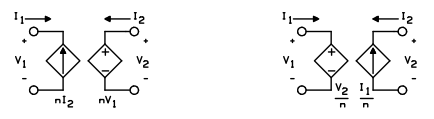
\includegraphics[width=(\textwidth-2cm)]{ideal_transformer_equiv.png}
	\end{center}
	\caption{
		Two equivalent circuits for an ideal transformer.
	}
	\label{FIG_IDEAL_TRANS_EQUIV}
\end{figure}
The relationships could be included in the powerflow equations specially, but more commonly real transformers are used, as described below; these may be expressed in the nodal admittance formalism.

A real transformer includes a leakage impedance (due to finite resistance of copper windings and core losses) and a shunt magnetising impedance. The latter is often large and may often be ignored. The nodal admittance matrix may be then derived:
\begin{align}
\begin{bmatrix}I_A \\ I_B \end{bmatrix} &= 
\begin{bmatrix}y_l/|a|^2 & -y_l/a^* \\ -y_l/a & y_l\end{bmatrix}
\begin{bmatrix}V_P \\ V_S \end{bmatrix}
\end{align}
where $a = V_P / V_S = N_P / N_S$ for an ideal transformer.

\subsection{Three-phase transformers}
The nodal admittance matrices of three-phase transformers may be derived from the single-phase expression, above, combined with information about the connections between phases.
\subsubsection{Delta-GWye}
\begin{figure}
\begin{center}
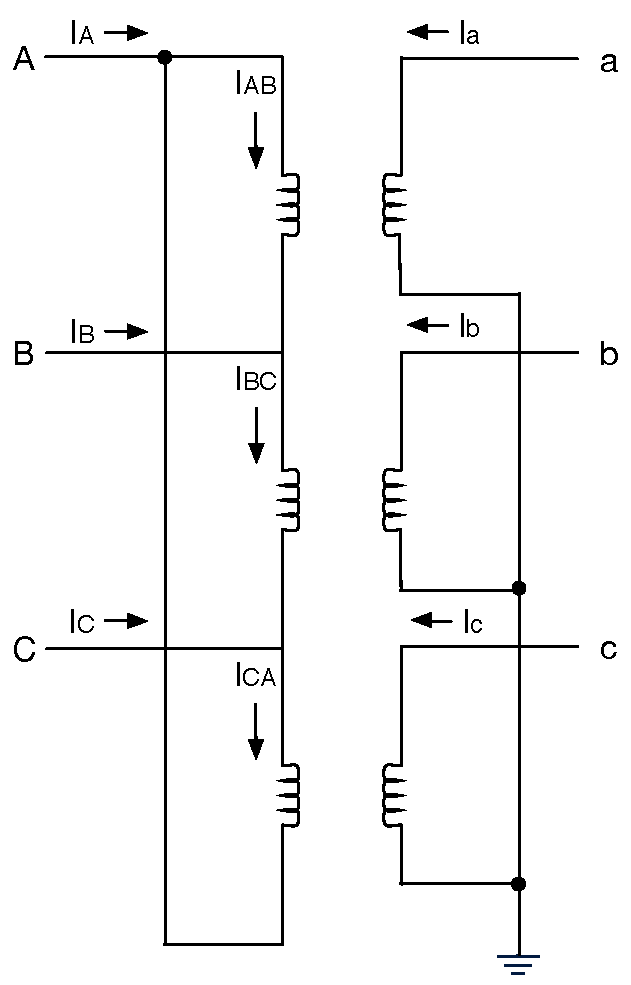
\includegraphics[width=7cm]{DeltaGWye.pdf}
\caption{Schematic of a Delta-GWye transformer}
\label{FIG_DELTA_GWYE}
\end{center}
\end{figure}
Considering Fig. \ref{FIG_DELTA_GWYE}, we have,
\begin{align}
I_{AB} &= \frac{y_l}{|a|^2}(V_A - V_B) - \frac{y_l}{a^*}V_a \\
I_{BC} &= \frac{y_l}{|a|^2}(V_B - V_C) - \frac{y_l}{a^*}V_b \\
I_{CA} &= \frac{y_l}{|a|^2}(V_C - V_A) - \frac{y_l}{a^*}V_c \\
I_a &= -\frac{y_l}{a}(V_A - V_B) + y_l V_a \\
I_b &= -\frac{y_l}{a}(V_B - V_C) + y_l V_b \\
I_c &= -\frac{y_l}{a}(V_C - V_A) + y_l V_c \\
\end{align}
Also, by the KCL, we have
\begin{align}
I_A &= I_{AB} - I_{CA} \\
&= \frac{y_l}{|a|^2}(2V_A - V_B - V_C) + \frac{y_l}{a^*}(V_c - V_a) \\
I_B &= I_{BC} - I_{AB} \\
&= \frac{y_l}{|a|^2}(2V_B - V_C - V_A) + \frac{y_l}{a^*}(V_a - V_b) \\
I_C &= I_{CA} - I_{BC} \\
&= \frac{y_l}{|a|^2}(2V_C - V_A - V_B) + \frac{y_l}{a^*}(V_b - V_c)
\end{align}
So we can immediately write down the nodal admittance relationship:
\begin{align}
\begin{bmatrix}I_A \\ I_B \\ I_C \\ I_a \\ I_b \\ I_c\end{bmatrix} &=
y_l \begin{bmatrix}
	2/|a|^2 & -1/|a|^2 & -1/|a|^2 & -1/a^* & 0 & 1/a^* \\
	-1/|a|^2 & 2/|a|^2 &  -1/|a|^2 & 1/a^*  & -1/a^* & 0 \\
	-1/|a|^2 &  -1/|a|^2 & 2/|a|^2 & 0 & 1/a^*  & -1/a^* \\
	-1/a & 1/a & 0 & 1 & 0 & 0 \\
	0 & -1/a & 1/a & 0 & 1 & 0 \\
	1/a & 0 & -1/a & 0 & 0 & 1
\end{bmatrix}
\begin{bmatrix}V_A \\ V_B \\ V_C \\ V_a \\ V_b \\ V_c\end{bmatrix}
\end{align}
with the nodal admittance matrix being specified by the matrix on the right, including the factor of $y_l$.
\section{The per-unit system}
There is a single MVA base power defined for the entire network. Power is expressed in units of this power.

Each bus has its own base voltage (usually expressed as Kv base). Bus voltages are then expressed in units of this voltage.

Current injections at a bus $i$ are expressed in units of $I_\text{base} = P_{base}/V_{\text{base},i}$. Thus care needs to be taken when translating current from one end of a line to the other end.

Impedances are expressed 
\end{document}